\documentclass[tikz,border=6pt]{standalone}
% shared TikZ style for the diagrams (colours match the plots)
\usepackage[T1]{fontenc}
\usepackage{lmodern}
\usepackage{amsmath,amssymb}
\usepackage{tikz}
\usetikzlibrary{arrows.meta,positioning,fit,backgrounds,calc,shapes.misc,decorations.pathreplacing}
\definecolor{cBlue}{HTML}{2A78D6}
\definecolor{cOrange}{HTML}{EB6834}
\definecolor{cAqua}{HTML}{1BAF7A}
\definecolor{cViolet}{HTML}{6250D6}
\definecolor{cGreen}{HTML}{008300}
\definecolor{cGray}{HTML}{8F8D86}
\definecolor{cInk}{HTML}{0B0B0B}
\definecolor{cInk2}{HTML}{52514E}
\tikzset{
  box/.style={draw=#1!70!black, fill=#1!10, rounded corners=3pt, align=center, inner sep=4pt, font=\small, line width=0.6pt},
  box/.default=cGray,
  arr/.style={-{Stealth[length=2.4mm]}, line width=0.8pt, cInk2},
  lbl/.style={font=\scriptsize, text=cInk2, align=center},
}

\begin{document}
\hyphenpenalty=10000\exhyphenpenalty=10000
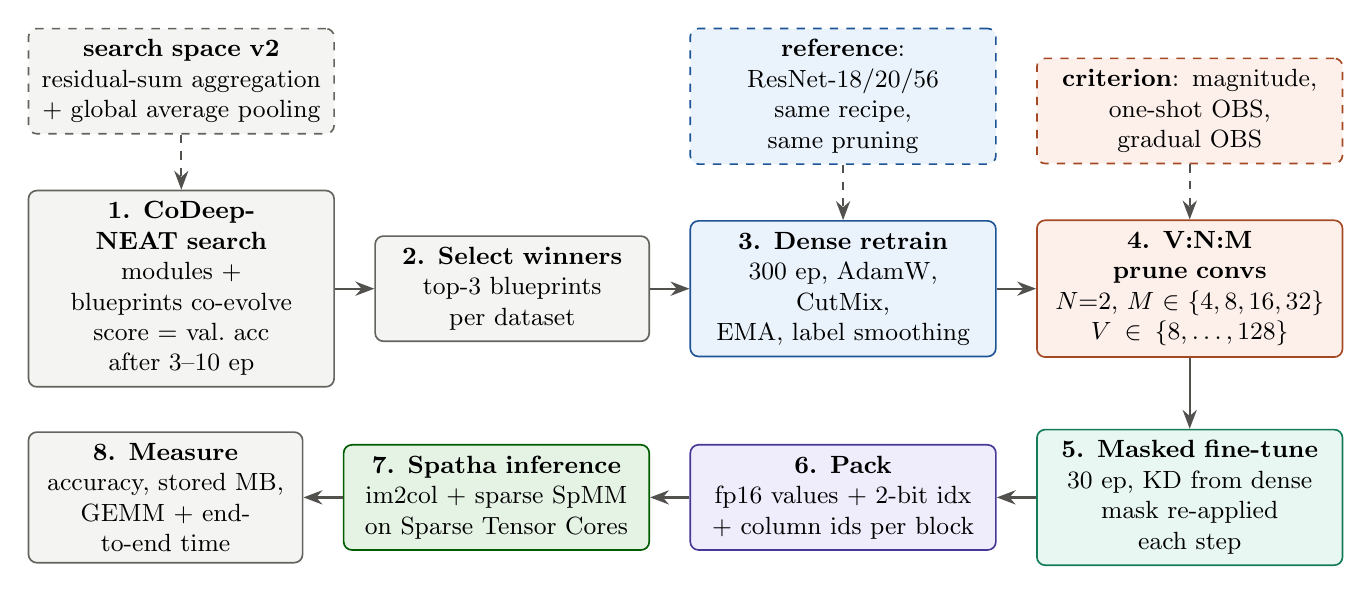
\begin{tikzpicture}[node distance=7mm and 5mm]
\node[box=cGray, text width=36mm] (evo) {\textbf{1. CoDeepNEAT search}\\modules + blueprints co-evolve\\score = val.\ acc after 3--10 ep};
\node[box=cGray, text width=32mm, right=of evo] (top) {\textbf{2. Select winners}\\top-3 blueprints\\per dataset};
\node[box=cBlue, text width=36mm, right=of top] (rt) {\textbf{3. Dense retrain}\\300 ep, AdamW, CutMix,\\EMA, label smoothing};
\node[box=cOrange, text width=36mm, right=of rt] (pr) {\textbf{4. V:N:M prune convs}\\$N{=}2$, $M\in\{4,8,16,32\}$\\$V\in\{8,\dots,128\}$};
\node[box=cAqua, text width=36mm, below=9mm of pr] (ft) {\textbf{5. Masked fine-tune}\\30 ep, KD from dense\\mask re-applied each step};
\node[box=cViolet, text width=36mm, left=of ft] (pk) {\textbf{6. Pack}\\fp16 values + 2-bit idx\\+ column ids per block};
\node[box=cGreen, text width=36mm, left=of pk] (sp) {\textbf{7. Spatha inference}\\im2col + sparse SpMM\\on Sparse Tensor Cores};
\node[box=cGray, text width=32mm, left=of sp] (ev) {\textbf{8. Measure}\\accuracy, stored MB,\\GEMM + end-to-end time};
\draw[arr] (evo)--(top); \draw[arr] (top)--(rt); \draw[arr] (rt)--(pr); \draw[arr] (pr)--(ft);
\draw[arr] (ft)--(pk); \draw[arr] (pk)--(sp); \draw[arr] (sp)--(ev);
\node[box=cGray, dashed, text width=36mm, above=7mm of evo] (ss) {\textbf{search space v2}\\residual-sum aggregation\\+ global average pooling};
\draw[arr, dashed] (ss)--(evo);
\node[box=cOrange, dashed, text width=36mm, above=7mm of pr] (crit) {\textbf{criterion}: magnitude,\\one-shot OBS, gradual OBS};
\draw[arr, dashed] (crit)--(pr);
\node[box=cBlue, dashed, text width=36mm, above=7mm of rt] (rn) {\textbf{reference}: ResNet-18/20/56\\same recipe, same pruning};
\draw[arr, dashed] (rn)--(rt);
\end{tikzpicture}
\end{document}
